% Template for PLoS
% Version 3.5 March 2018
%
% % % % % % % % % % % % % % % % % % % % % %
%
% -- IMPORTANT NOTE
%
% This template contains comments intended
% to minimize problems and delays during our production
% process. Please follow the template instructions
% whenever possible.
%
% % % % % % % % % % % % % % % % % % % % % % %
%
% Once your paper is accepted for publication,
% PLEASE REMOVE ALL TRACKED CHANGES in this file
% and leave only the final text of your manuscript.
% PLOS recommends the use of latexdiff to track changes during review, as this will help to maintain a clean tex file.
% Visit https://www.ctan.org/pkg/latexdiff?lang=en for info or contact us at latex@plos.org.
%
%
% There are no restrictions on package use within the LaTeX files except that
% no packages listed in the template may be deleted.
%
% Please do not include colors or graphics in the text.
%
% The manuscript LaTeX source should be contained within a single file (do not use \input, \externaldocument, or similar commands).
%
% % % % % % % % % % % % % % % % % % % % % % %
%
% -- FIGURES AND TABLES
%
% Please include tables/figure captions directly after the paragraph where they are first cited in the text.
%
% DO NOT INCLUDE GRAPHICS IN YOUR MANUSCRIPT
% - Figures should be uploaded separately from your manuscript file.
% - Figures generated using LaTeX should be extracted and removed from the PDF before submission.
% - Figures containing multiple panels/subfigures must be combined into one image file before submission.
% For figure citations, please use "Fig" instead of "Figure".
% See http://journals.plos.org/plosone/s/figures for PLOS figure guidelines.
%
% Tables should be cell-based and may not contain:
% - spacing/line breaks within cells to alter layout or alignment
% - do not nest tabular environments (no tabular environments within tabular environments)
% - no graphics or colored text (cell background color/shading OK)
% See http://journals.plos.org/plosone/s/tables for table guidelines.
%
% For tables that exceed the width of the text column, use the adjustwidth environment as illustrated in the example table in text below.
%
% % % % % % % % % % % % % % % % % % % % % % % %
%
% -- EQUATIONS, MATH SYMBOLS, SUBSCRIPTS, AND SUPERSCRIPTS
%
% IMPORTANT
% Below are a few tips to help format your equations and other special characters according to our specifications. For more tips to help reduce the possibility of formatting errors during conversion, please see our LaTeX guidelines at http://journals.plos.org/plosone/s/latex
%
% For inline equations, please be sure to include all portions of an equation in the math environment.
%
% Do not include text that is not math in the math environment.
%
% Please add line breaks to long display equations when possible in order to fit size of the column.
%
% For inline equations, please do not include punctuation (commas, etc) within the math environment unless this is part of the equation.
%
% When adding superscript or subscripts outside of brackets/braces, please group using {}.
%
% Do not use \cal for caligraphic font.  Instead, use \mathcal{}
%
% % % % % % % % % % % % % % % % % % % % % % % %
%
% Please contact latex@plos.org with any questions.
%
% % % % % % % % % % % % % % % % % % % % % % % %

\documentclass[10pt,letterpaper]{article}
\usepackage[top=0.85in,left=2.75in,footskip=0.75in]{geometry}

% amsmath and amssymb packages, useful for mathematical formulas and symbols
\usepackage{amsmath,amssymb}

% Use adjustwidth environment to exceed column width (see example table in text)
\usepackage{changepage}

% Use Unicode characters when possible
\usepackage[utf8x]{inputenc}

% textcomp package and marvosym package for additional characters
\usepackage{textcomp,marvosym}

% cite package, to clean up citations in the main text. Do not remove.
% \usepackage{cite}

% Use nameref to cite supporting information files (see Supporting Information section for more info)
\usepackage{nameref,hyperref}

% line numbers
\usepackage[right]{lineno}

% ligatures disabled
\usepackage{microtype}
\DisableLigatures[f]{encoding = *, family = * }

% color can be used to apply background shading to table cells only
\usepackage[table]{xcolor}

% array package and thick rules for tables
\usepackage{array}

% create "+" rule type for thick vertical lines
\newcolumntype{+}{!{\vrule width 2pt}}

% create \thickcline for thick horizontal lines of variable length
\newlength\savedwidth
\newcommand\thickcline[1]{%
  \noalign{\global\savedwidth\arrayrulewidth\global\arrayrulewidth 2pt}%
  \cline{#1}%
  \noalign{\vskip\arrayrulewidth}%
  \noalign{\global\arrayrulewidth\savedwidth}%
}

% \thickhline command for thick horizontal lines that span the table
\newcommand\thickhline{\noalign{\global\savedwidth\arrayrulewidth\global\arrayrulewidth 2pt}%
\hline
\noalign{\global\arrayrulewidth\savedwidth}}


% Remove comment for double spacing
%\usepackage{setspace}
%\doublespacing

% Text layout
\raggedright
\setlength{\parindent}{0.5cm}
\textwidth 5.25in
\textheight 8.75in

% Bold the 'Figure #' in the caption and separate it from the title/caption with a period
% Captions will be left justified
\usepackage[aboveskip=1pt,labelfont=bf,labelsep=period,justification=raggedright,singlelinecheck=off]{caption}
\renewcommand{\figurename}{Fig}

% Use the PLoS provided BiBTeX style
% \bibliographystyle{plos2015}

% Remove brackets from numbering in List of References
\makeatletter
\renewcommand{\@biblabel}[1]{\quad#1.}
\makeatother



% Header and Footer with logo
\usepackage{lastpage,fancyhdr,graphicx}
\usepackage{epstopdf}
%\pagestyle{myheadings}
\pagestyle{fancy}
\fancyhf{}
%\setlength{\headheight}{27.023pt}
%\lhead{
\includegraphics[width=2.0in]{PLOS-submission.eps}}
\rfoot{\thepage/\pageref{LastPage}}
\renewcommand{\headrulewidth}{0pt}
\renewcommand{\footrule}{\hrule height 2pt \vspace{2mm}}
\fancyheadoffset[L]{2.25in}
\fancyfootoffset[L]{2.25in}
\lfoot{\today}

%% Include all macros below

\newcommand{\lorem}{{\bf LOREM}}
\newcommand{\ipsum}{{\bf IPSUM}}

\usepackage{color}
\usepackage{fancyvrb}
\newcommand{\VerbBar}{|}
\newcommand{\VERB}{\Verb[commandchars=\\\{\}]}
\DefineVerbatimEnvironment{Highlighting}{Verbatim}{commandchars=\\\{\}}
% Add ',fontsize=\small' for more characters per line
\usepackage{framed}
\definecolor{shadecolor}{RGB}{248,248,248}
\newenvironment{Shaded}{\begin{snugshade}}{\end{snugshade}}
\newcommand{\AlertTok}[1]{\textcolor[rgb]{0.94,0.16,0.16}{#1}}
\newcommand{\AnnotationTok}[1]{\textcolor[rgb]{0.56,0.35,0.01}{\textbf{\textit{#1}}}}
\newcommand{\AttributeTok}[1]{\textcolor[rgb]{0.77,0.63,0.00}{#1}}
\newcommand{\BaseNTok}[1]{\textcolor[rgb]{0.00,0.00,0.81}{#1}}
\newcommand{\BuiltInTok}[1]{#1}
\newcommand{\CharTok}[1]{\textcolor[rgb]{0.31,0.60,0.02}{#1}}
\newcommand{\CommentTok}[1]{\textcolor[rgb]{0.56,0.35,0.01}{\textit{#1}}}
\newcommand{\CommentVarTok}[1]{\textcolor[rgb]{0.56,0.35,0.01}{\textbf{\textit{#1}}}}
\newcommand{\ConstantTok}[1]{\textcolor[rgb]{0.00,0.00,0.00}{#1}}
\newcommand{\ControlFlowTok}[1]{\textcolor[rgb]{0.13,0.29,0.53}{\textbf{#1}}}
\newcommand{\DataTypeTok}[1]{\textcolor[rgb]{0.13,0.29,0.53}{#1}}
\newcommand{\DecValTok}[1]{\textcolor[rgb]{0.00,0.00,0.81}{#1}}
\newcommand{\DocumentationTok}[1]{\textcolor[rgb]{0.56,0.35,0.01}{\textbf{\textit{#1}}}}
\newcommand{\ErrorTok}[1]{\textcolor[rgb]{0.64,0.00,0.00}{\textbf{#1}}}
\newcommand{\ExtensionTok}[1]{#1}
\newcommand{\FloatTok}[1]{\textcolor[rgb]{0.00,0.00,0.81}{#1}}
\newcommand{\FunctionTok}[1]{\textcolor[rgb]{0.00,0.00,0.00}{#1}}
\newcommand{\ImportTok}[1]{#1}
\newcommand{\InformationTok}[1]{\textcolor[rgb]{0.56,0.35,0.01}{\textbf{\textit{#1}}}}
\newcommand{\KeywordTok}[1]{\textcolor[rgb]{0.13,0.29,0.53}{\textbf{#1}}}
\newcommand{\NormalTok}[1]{#1}
\newcommand{\OperatorTok}[1]{\textcolor[rgb]{0.81,0.36,0.00}{\textbf{#1}}}
\newcommand{\OtherTok}[1]{\textcolor[rgb]{0.56,0.35,0.01}{#1}}
\newcommand{\PreprocessorTok}[1]{\textcolor[rgb]{0.56,0.35,0.01}{\textit{#1}}}
\newcommand{\RegionMarkerTok}[1]{#1}
\newcommand{\SpecialCharTok}[1]{\textcolor[rgb]{0.00,0.00,0.00}{#1}}
\newcommand{\SpecialStringTok}[1]{\textcolor[rgb]{0.31,0.60,0.02}{#1}}
\newcommand{\StringTok}[1]{\textcolor[rgb]{0.31,0.60,0.02}{#1}}
\newcommand{\VariableTok}[1]{\textcolor[rgb]{0.00,0.00,0.00}{#1}}
\newcommand{\VerbatimStringTok}[1]{\textcolor[rgb]{0.31,0.60,0.02}{#1}}
\newcommand{\WarningTok}[1]{\textcolor[rgb]{0.56,0.35,0.01}{\textbf{\textit{#1}}}}


\usepackage[user,titleref]{zref}
\newcommand*{\rulelabel}[2]{\ztitlerefsetup{title=#1} \zlabel{#2} \label{#2} \zrefused{#2}}
\newcommand*{\ruleref}[1]{\hyperref[{#1}]{Rule~\ztitleref{#1}}}



\usepackage{forarray}
\usepackage{xstring}
\newcommand{\getIndex}[2]{
  \ForEach{,}{\IfEq{#1}{\thislevelitem}{\number\thislevelcount\ExitForEach}{}}{#2}
}

\setcounter{secnumdepth}{0}

\newcommand{\getAff}[1]{
  \getIndex{#1}{}
}

\providecommand{\tightlist}{%
  \setlength{\itemsep}{0pt}\setlength{\parskip}{0pt}}

\begin{document}
\vspace*{0.2in}

% Title must be 250 characters or less.
\begin{flushleft}
{\Large
\textbf\newline{Ten Simple Rules for Writing Dockerfiles for Reproducible Data Science} % Please use "sentence case" for title and headings (capitalize only the first word in a title (or heading), the first word in a subtitle (or subheading), and any proper nouns).
}
\newline
% Insert author names, affiliations and corresponding author email (do not include titles, positions, or degrees).
\\
Daniel Nüst\textsuperscript{\getAff{Institute for Geoinformatics, University of Muenster, Muenster, Germany}}\textsuperscript{*},
Vanessa Sochat\textsuperscript{\getAff{Stanford Research Computing Center, Stanford University, Stanford, CA,
US}},
Ben Marwick\textsuperscript{\getAff{Department of Anthropology, University of Washington, Seattle, USA}},
Stephen J. Eglen\textsuperscript{\getAff{Department of Applied Mathematics and Theoretical Physics, University of
Cambridge, Cambridge, Cambridgeshire, GB}},
Tim Head\textsuperscript{\getAff{Wild Tree Tech, Zurich, CH}},
Tony Hirst\textsuperscript{\getAff{Department of Computing and Communications, The Open University, GB}}\\
\bigskip
\bigskip
* Corresponding author: daniel.nuest@uni-muenster.de\\
\end{flushleft}
% Please keep the abstract below 300 words
\section*{Abstract}
Containers are greatly improving computational science by packaging
software and data dependencies. In a scholarly context, transparency and
support of reproducibility are the largest drivers for using these
containers. It follows that choices that are made with respect to
building containers can make or break a workflow's reproducibility. The
build for the container image is often created based on the instructions
in the \texttt{Dockerfile} format. The rules presented here help
researchers to write understandable \texttt{Dockerfile}s for typical
data science workflows. By following the rules in this article
researchers can create containers suitable for sharing with fellow
scientists, for inclusion in scholarly communication such as education
or scientific papers, and for an effective and sustainable personal
workflow.

% Please keep the Author Summary between 150 and 200 words
% Use first person. PLOS ONE authors please skip this step.
% Author Summary not valid for PLOS ONE submissions.

\linenumbers

% Use "Eq" instead of "Equation" for equation citations.
\hypertarget{introduction}{%
\section*{Introduction}\label{introduction}}
\addcontentsline{toc}{section}{Introduction}

Computing infrastructure has advanced to the point where not only can we
share data underlying research articles, we can share the code that
processes these data. This sharing of code files is enabled by
collaboration platforms such as \href{https://github.com}{GitHub} or
\href{https://gitlab.com}{GitLab} and has become quite common. The
sharing of the computing environment, on the other hand, is enabled by
containerization, which allows for documenting and sharing entire
workflows in a comprehensive way. This sharing of computational assets
is paramount to increasing the reproducibility of computational
research. While ``papers'' based on the traditional journal article
format can share high level details of research, computational research
is oftentimes way too complicated to be disseminated alongside in this
format {[}1{]}. In that the actual contribution to knowledge includes
the full computing environment that produced a result {[}2{]},
containerization is needed.

Containerization plays an important role in providing instructions for
packaging the building blocks of computer-based research (i.e.~code,
data, documentation, and the computing environment). Containers are
built from plain text files that represent a human- \emph{and}
machine-readable recipe for creating the computing environment and
interacting with data. By providing this recipe, authors of scientific
articles greatly improve their work's level of documentation,
transparency, and reusability. Specification of the computing
environment is an important and common practice in scientific computing
{[}3,4{]}, with the result that it is much more likely that both the
author and others are able to reproduce and extend an analysis workflow.
The containers built from these recipes are portable encapsulated
snapshots of a specific computing environment. Such containers have been
demonstrated for capturing scientific notebooks {[}5{]} and reproducible
workflows {[}6{]}.

While there are several tutorials for using containers for reproducible
research {[}7--11{]}, there is no detailed \emph{manual for how to write
the actual instructions to create the containers for computational
research} besides generic best practices {[}12,13{]}. Guening et~al.
{[}14{]} give very helpful recommendations for packaging reusable
software in a container. This article introduces these instructions for
the popular \texttt{Dockerfile} format with a focus on containers
encapsulating data science workflows.

\hypertarget{prerequisites-scope}{%
\section{Prerequisites \& scope}\label{prerequisites-scope}}

To start with, we assume you have a scripted scientific workflow,
i.e.~you can, at least at a certain point in time, execute the full
process with a fixed set of commands, for example
\texttt{make\ prepare\_data} followed by \texttt{Rscript\ analysis.R},
or only \texttt{python3\ my-workflow.py}. Since containers that you
eventually share with others can only run open source software, tools
like Mathematica and Matlab are out of scope for this example. A
workflow that does not support scripted execution is also out of scope
for reproducible research, as it does not fit well with
containerization. Furthermore, workflows interacting with many petabytes
of data and executed in high-performance computing (HPC) infrastructures
are out of scope. Using such HPC job managers or cloud infrastructures
would require a collection of ``Ten Simple Rules'' articles in their own
right. For this article, we focus on workflows that typically run on
single machine, e.g., a researchers laptop computer or a virtual server.
The reader might scope the data requirement to less than a terabyte, and
compute requirement to a machine with 16 cores running over the weekend.

While out of scope for this article, we point the reader to
\texttt{docker-compose} {[}15{]} in the case of needing container
orchestration for multiple applications, e.g., web servers, databases,
and worker containers. A \texttt{docker-compose.yml} configuration file
allows for defining volumes, environment variables, and exposed ports
and helps to stick to \emph{one purpose per container}, which often
means one process running in the container, and to combine existing
stable building blocks instead of bespoke massive containers for
specific purposes.

Because \emph{``the number of unique research environments approximates
the number of researchers''} {[}16{]}, sticking to conventions helps
every researcher to understand, modify, and eventually write container
recipes suitable for their needs. Even if they are not sure how the
technology behind them actually works, researchers should leverage
containerization following good practices. The practices that are to be
discussed in this article are strongly related to software engineering
in general and research software engineering (RSEng) in particular,
which is concerned with quality, training, and recognition of software
in science {[}17{]}. Research Software Engineers (RSEs) are not the
target audience for this work, but we want to encourage you to reach out
to your local or national RSE community if your needs go beyond the
rules of this work.

While there are many different container technologies, this article
focuses on Docker {[}18{]}. Docker is a highly suitable tool for
reproducible research (e.g., {[}19{]}) and our observations indicate it
is the most widely used container technology in academic data science.
The goal of this article is to guide you to write a \texttt{Dockerfile},
which is a file format for creating container images. The rules help you
to ensure the \texttt{Dockerfile} allows for interactive development as
well as the higher goals of reproducibility and preservation of
knowledge. Such practices are generally not part of generic
containerization tutorials and are rarely found in \texttt{Dockerfile}s
published as part of software projects, which are often used as
templates by novices. The differences between a helpful, stable
\texttt{Dockerfile} and one that is misleading, prone to failure, and
full of potential obstacles, are not obvious, especially for researchers
who do not have extensive software development experience or formal
training. A commitment to this article's rules can ensure that workflows
are reproducible and reusable, that computing environments are
understandable by others, and researchers can collaborate effectively.
Their application should not be triggered by the publication of a
finished project, but be weaved into day-to-day habits (cf.~thoughts on
openness as an afterthought by {[}20{]} and on computational
reproducibility by {[}2{]}).

\hypertarget{docker-dockerfiles}{%
\section{Docker \& Dockerfiles}\label{docker-dockerfiles}}

Docker {[}18{]} is a container technology that is widely adopted and
supported on many platforms, and has become highly useful for research.
Containers are distinct from virtual machines (VM) or hypervisors as
they do not emulate hardware or operating system kernels, and thus do
not require the same system resources. Several solutions for
facilitating reproducible research are built on top of containers
{[}16,21--24{]}, but they intentionally hide most of the complexity from
the researcher.

To create Docker containers for specific workflows, we write text files
that follow a particular format called \texttt{Dockerfile} {[}25{]}.
\texttt{Dockerfile}s are machine- \emph{and} human-readable recipes for
building images, comparable to Makefiles {[}26{]}. Container images
include the application, e.g., the programming language interpreter
needed to run a workflow, and the system libraries required by an
application to run. A \texttt{Dockerfile} consists of a sequence of
instructions to copy files and install software. Each instruction adds a
layer to the image, which can be cached across image builds for
minimizing build and download times. The images have a main executable
exposed as an ``entrypoint'' that is started when they are run as
stateful containers, which are the running instances of Docker images.
Containers can be modified, stopped, restarted and purged. A visual
analogy for building and running a container is provided in Figure~1.
Akin to compiling source code for a programming language, creating a
container also starts with a plain text file (Dockerfile), which
provides instructions for building an image. Similarly to using a
compiled binary file to launch a program, the image is then run to
create a container instance. See Listing~1 for a full
\texttt{Dockerfile}, which we will refer to throughout this article.

\begin{figure}
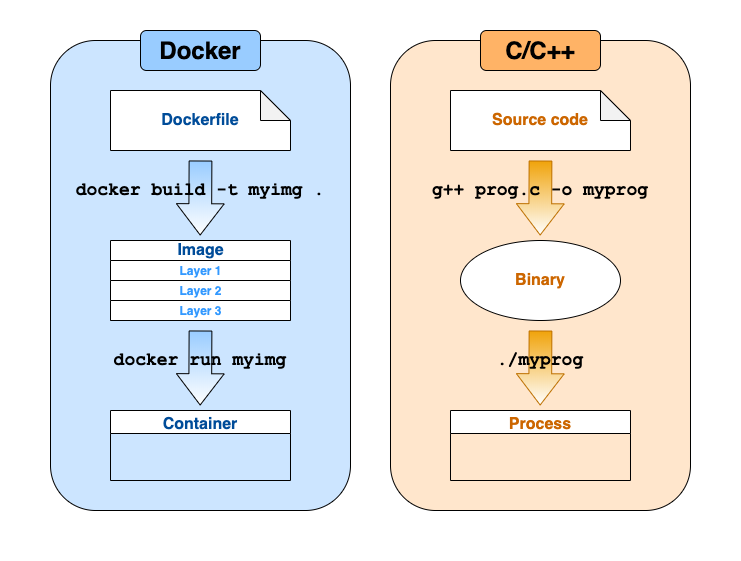
\includegraphics[width=1\linewidth]{container-analogy} \caption{The workflow to create Docker containers by analogy. Containers begin with a Dockerfile, a recipe for building the computational environment (analogous to source code in a compiled programming language). This is used to build an image with the `docker build` command (analogous to compiling the source code into a binary). Finally the image is used to launch one or more containers with the `docker run` command (analogous to running an instance of the compiled binary as a process).}\label{fig:container-analogy}
\end{figure}

While Docker was the original technology to support the
\texttt{Dockerfile} format, other container technologies with support
include
\href{https://podman.io/}{podman}/\href{https://github.com/containers/buildah}{buildah}
supported by RedHat,
\href{https://github.com/GoogleContainerTools/kaniko}{kaniko},
\href{https://github.com/genuinetools/img}{img}, and
\href{https://github.com/moby/buildkit}{buildkit}. The Singularity
container software {[}27{]} is optimised for high performance computing
and although it uses its own format, the \emph{Singularity recipe}, it
can import and run Docker images. Although the Singularity recipe format
is different, the rules here are transferable to some extent. While some
may argue for reasons to not publish reproducibly, e.g., lack of time
and incentives, reluctance to share (cf.~{[}28{]}) and there are
substantial technical challenges to maintain software and documentation,
providing a \texttt{Dockerfile}, a pre-built Docker image, or other type
of container should become an increasingly easier task for the average
researcher. If a researcher is able to find and create containers or
write a \texttt{Dockerfile} to address their most common use cases, then
arguably it will not be extra work after this initial set up (cf.~README
of {[}29{]}). In fact, the \texttt{Dockerfile} itself can be a powerful
documentation to show from where data and code was derived,
i.e.~downloaded or installed, and consequently where a third party might
obtain them again.

\footnotesize

\begin{Shaded}
\begin{Highlighting}[]
\KeywordTok{FROM}\NormalTok{ rocker/verse:3.6.2}

\CommentTok{# install Java, needed for package rJava}
\KeywordTok{RUN}\NormalTok{ apt-get update \textbackslash{}}
\NormalTok{  && apt-get install -y default-jdk \textbackslash{}}
\NormalTok{  && rm -rf /var/lib/apt/lists/*}

\CommentTok{# install system dependencies for R packages}
\KeywordTok{RUN}\NormalTok{ apt-get update \textbackslash{}}
\NormalTok{  && apt-get install}
    \CommentTok{# needed for RNetCDF:}
\NormalTok{    netcdf udunits-2 \textbackslash{}}
    \CommentTok{# needed for ...:}
\NormalTok{    more \textbackslash{}}
\NormalTok{    arguments}

\CommentTok{# Taken from https://github.com/rocker-org/geospatial/blob/master/Dockerfile}
\KeywordTok{RUN}\NormalTok{ install2.r --error \textbackslash{}}
\NormalTok{    RColorBrewer \textbackslash{}}
\NormalTok{    RandomFields \textbackslash{}}
\NormalTok{    RNetCDF}

\KeywordTok{WORKDIR}\NormalTok{ /tmp}
    
\CommentTok{# Install latest version of crucial tool with bugfix from source}
\KeywordTok{RUN}\NormalTok{ apt-get update \textbackslash{}}
\NormalTok{  && apt-get install -y \textbackslash{}}
\NormalTok{    build-essential \textbackslash{}}
\NormalTok{  && wget https://download.url/crucialware/version-1.2.3.zip \textbackslash{}}
\NormalTok{  && unzip *.zip -d crucialware \textbackslash{}}
\NormalTok{  && cd crucialware \textbackslash{}}
\NormalTok{  && ./configure && make && make install \textbackslash{}}
\NormalTok{  && rm -rf /tmp/crucialware version-*.zip \textbackslash{}}
\NormalTok{  && rm -rf /var/lib/apt/lists/*}
  
\CommentTok{# Install Python tools}
\KeywordTok{COPY}\NormalTok{ requirements.txt requirements.txt}
\KeywordTok{RUN}\NormalTok{ pip install -r requirements.txt}

\CommentTok{# Add workflow scripts}
\KeywordTok{WORKDIR}\NormalTok{ /work}
\KeywordTok{COPY}\NormalTok{ myscript.sh myscript.sh}
\KeywordTok{COPY}\NormalTok{ plots.R plots.R}

\CommentTok{# Uncomment the following lines to execute preprocessing and processing tasks during build}
\CommentTok{#RUN snakemake --use-conda <other params>}
\CommentTok{#RUN nextflow workflow.nf --in 'dataset/*.fa'}
\CommentTok{#RUN java -jar cromwell-XY.jar run myWorkflow.wdl}
\CommentTok{#RUN Rscript plots.R}

\CommentTok{# CMD from base image used for development, uncomment the following lines to have a }
\CommentTok{# "run workflow only" container}
\CommentTok{# CMD["./myscript.sh"]}

\CommentTok{### Usage instructions }\AlertTok{###}
\CommentTok{# Build the images with}
\CommentTok{# > docker build --tag great_workflow:1.0.0 .}
\CommentTok{# Run the image:}
\CommentTok{# > docker run --it --port 80:8787 --volume ./input:/input \textbackslash{}}
\CommentTok{#     --name gwf great_workflow}
\CommentTok{# Extract the data:}
\CommentTok{# > docker cp gwf:/output/ ./outputData}
\CommentTok{# Extract the figures:}
\CommentTok{# > docker cp gwf:/work/figures/ ./figures}
\end{Highlighting}
\end{Shaded}

\normalsize

\emph{Listing~1}: \texttt{Dockerfile} full example.

\hypertarget{consider-tools-to-assist-with-dockerfile-generation}{%
\section*{1. Consider tools to assist with Dockerfile
generation}\label{consider-tools-to-assist-with-dockerfile-generation}}
\addcontentsline{toc}{section}{1. Consider tools to assist with
Dockerfile generation}

\ztitlerefsetup{title=1} \zlabel{rule:tools} \label{rule:tools} \zrefused{rule:tools}

Rule 1 could informally be described as ``Don't bother to write a
Dockerfile!''. Writing a \texttt{Dockerfile} from scratch can be
difficult and even experts sometimes take shortcuts. Thus, it is a good
strategy to first look to tools that can help to generate a
\texttt{Dockerfile} for you. Such tools have likely thought about and
implemented good practices, and they may have added newer practices when
reapplied at a later point in time. Therefore the most important rule is
to apply a multi-step process for your specific use case.

First, you want to determine if there is an already existing container
that you can use, and in this case, use it and add to your workflow
documentation instructions for doing so. As an example, you might be
doing some kind of interactive development. For interactive development
environments such as notebooks and development servers or databases, you
can readily find containers that come installed with all the software
that you need. You can look for information about images in (a) the
documentation of the used software, (b) the Docker image registry
\emph{Docker Hub}, \url{https://hub.docker.com/}, or (c) the source code
projects of the used software, as many developers today rely on
containers for development, testing, and teaching.

Second, in the case that there is no suitable pre-existing container for
your needs, you might next look to well-maintained tools to help with
\texttt{Dockerfile} generation. These tools can add required software
packages to an existing image without you having to manually write a
\texttt{Dockerfile} at all. ``Well-maintained'' references the tool's
own stability and usability, but also that suitable base images are
used, likely from the official Docker library {[}30{]}, to ensure that
the container has the most recent security fixes for the operating
system in question. See below box ``Tools for container generation'' for
details.

Third, you may want to write you own \texttt{Dockerfile} if these tools
do not suffice for your needs. \emph{In this case, follow the remaining
rules.}

\begin{center}\rule{0.5\linewidth}{0.5pt}\end{center}

\hypertarget{tools-for-container-generation}{%
\subsection{Tools for container
generation}\label{tools-for-container-generation}}

Repo2docker {[}24{]} is a tool that is maintained by
\href{https://jupyter.org/}{Project Jupyter} that can help to transform
a source code or data repository, e.g.~GitHub, GitLab, or Zenodo, into a
container. The tool relies on common configuration files for defining
software dependencies and versions, and supports a few more special
files for, see the
\href{https://repo2docker.readthedocs.io/en/latest/config_files.html}{supported
configuration files}. As an example, we might install
\texttt{jupyter-repo2docker} and then run it against a repository with a
\texttt{requirements.txt} file, an indication of being a Python workflow
with dependencies on the \href{https://pypi.org/}{Python Package Index}
(PyPI) with the following command.

\footnotesize

\begin{Shaded}
\begin{Highlighting}[]
\ExtensionTok{jupyter-repo2docker}\NormalTok{ https://github.com/norvig/pytudes}
\end{Highlighting}
\end{Shaded}

\normalsize

The resulting container image installs the dependencies listed in the
requirements file, along with providing an entrypoint to run a notebook
server to interact with any existing workflows in the repository. Since
repo2docker is used within \href{https://mybinder.org/}{MyBinder.org},
if you make sure your workflow is ``Binder-ready'', you and others can
also get an online workspace with a single click. A precaution that
needs to be taken is that the default command above will create a home
for the current user, meaning that the container itself would not be
ideal to share, but rather any researchers interested in interaction
with the code inside should run repo2docker themselves and create their
own container. Because repo2docker is deterministic, the environments
are the same
(see~\hyperref[{rule:pinning}]{Rule~\ztitleref{rule:pinning}} for
ensuring the same software versions).

Additional tools to assist with writing \texttt{Dockerfile}s include
\texttt{containerit} {[}31{]} and \texttt{dockta} {[}32{]}.
\texttt{containerit} automates the generation of standalone
\texttt{Dockerfile}s for workflows in R. It can provide a starting point
for users unfamiliar with writing \texttt{Dockerfile}s, or together with
other R packages provide a full image creation and execution process
without having to leave an R session. \texttt{dockta} supports multiple
programming languages and configurations files, just as
\texttt{repo2docker}, but attempts to create readable
\texttt{Dockerfile}s compatible with plain Docker and to improve user
experience by cleverly adjusting instructions to reduce build time. For
any tool that you use, be sure to look at documentation for usage and
configuration options, and options to add metadata (e.g., labels
see~\hyperref[{rule:document}]{Rule~\ztitleref{rule:document}}).

\begin{center}\rule{0.5\linewidth}{0.5pt}\end{center}

\hypertarget{use-versioned-images}{%
\section*{2. Use versioned images}\label{use-versioned-images}}
\addcontentsline{toc}{section}{2. Use versioned images}

\ztitlerefsetup{title=2} \zlabel{rule:base} \label{rule:base} \zrefused{rule:base}

A good understanding of how base images and image tags work is crucial,
as the image and tag that you choose has important implications for your
container. It is good practice to use base images that are maintained by
the Docker library, so called \emph{``official images''} {[}33{]}, which
benefit from a review for best practices and vulnerability scanning
{[}12{]}. You can identify these images by the missing the user portion
of the image name, which comes before the \texttt{/}, e.g.,
\texttt{r-base} or \texttt{python}. However, these images only provide
basic programming languages or very widely used software, so you will
likely use images maintained by organizations or fellow researchers.
While some organizations can be trusted to update containers with
security fixes (see list below), for most individual accounts that
provide ready to use images, it is likely that these will not be updated
regularly. It is even possible that images or \texttt{Dockerfile}s may
disappear, or that images are published with malicious intent, though we
have not heard of any such case in academia. Therefore, for security,
transparency, and reproducibility, you should only use images where you
have access to the \texttt{Dockerfile}, and it is suggested to save a
copy of the \texttt{Dockerfile} in the case that a repository or other
distribution goes away.

Images have \emph{tags} associated with them with specific meanings,
e.g., a version indicator such as \texttt{3.7} or \texttt{dev}, or
variants such as \texttt{slim} attempting to reduce image size. Tags are
defined at image build time and appear in image name after the
\texttt{:} when you use an image, e.g., \texttt{python:3.7}. By
\emph{convention} a missing tag is assumed to be the word
\texttt{latest}, which gives you the latest updates but also a moving
target for your computing environment that can break your workflow. Note
that a version tag means that the tagged software is frozen, but it does
not mean the image will not change, as backwards compatible fixes
(cf.~semantic versioning, {[}34{]}), e.g., version \texttt{1.2.3} fixing
a security problem in version \texttt{1.2.2} or updates to an underlying
system library, would be published to the parent tag \texttt{1.2}.

For data science workflows, you should always rely on version-specific
image tags both for base images that you use, and for images that you
build yourself and then run. With keeping different versions (tags)
available, it is good practice to publish an image in an image registry.
We refer you to the documentation on automated builds for details, see
\href{https://docs.docker.com/docker-hub/builds/}{Docker Hub Builds} or
\href{https://docs.gitlab.com/ee/user/packages/container_registry/index.html\#build-and-push-images}{GitLab's
Container Registry} as well as continuous integration (CI) services such
as
\href{https://github.com/actions/starter-workflows/tree/master/ci}{GitHub
actions}, or
\href{https://circleci.com/orbs/registry/orb/circleci/docker\#commands-build}{CircleCI}
that can help you get started. Do not \texttt{docker\ push} a locally
built image, because that counteracts the considerations outlined above.
If a pre-built image is provided in a public image registry, do not
forget to direct the user to it in your documentation, e.g.~in the
\texttt{README} file or in an article.

The following list a selection of communities that produce widely used
regularly updated images, including ready-to-use images with
preinstalled software stacks. Do take advantage of images with complex
software environments pre-installed, e.g., machine learning tool stacks,
specific
\href{https://en.wikipedia.org/wiki/Basic_Linear_Algebra_Subprograms}{BLAS}
library.

\begin{itemize}
\tightlist
\item
  \href{https://www.rocker-project.org/}{Rocker} for R and RStudio
  images {[}19{]}
\item
  \href{https://bioconductor.org/help/docker/}{Bioconductor Docker
  images} for bioinformatics with R
\item
  \href{https://hub.docker.com/_/neurodebian}{NeuroDebian images} for
  neuroscience {[}35{]}
\item
  \href{https://jupyter-docker-stacks.readthedocs.io/en/latest/index.html}{Jupyter
  Docker Stacks} for Notebook-based computing
\item
  \href{https://hub.docker.com/r/taverna/taverna-server}{Taverna Server}
  for running Taverna workflows
\end{itemize}

For example, here is how we would use a base image \texttt{verse}, which
provides the popular Tidyverse suite of packages {[}36{]}, with R
version \texttt{3.5.2} from the \texttt{rocker} organization on Docker
Hub (\texttt{docker.io}, which is the default and can be omitted).

\footnotesize

\begin{Shaded}
\begin{Highlighting}[]
\KeywordTok{FROM}\NormalTok{ docker.io/rocker/r-ver:3.5.2}
\end{Highlighting}
\end{Shaded}

\normalsize

\hypertarget{format-intentionally-and-favor-clarity}{%
\section{3. Format intentionally and favor
clarity}\label{format-intentionally-and-favor-clarity}}

\ztitlerefsetup{title=3} \zlabel{rule:formatting} \label{rule:formatting} \zrefused{rule:formatting}
\ztitlerefsetup{title=3} \zlabel{rule:clarity} \label{rule:clarity} \zrefused{rule:clarity}

First, it is good practice to think of the \texttt{Dockerfile} as a
human \emph{and} machine readable file. This means that you should use
indentation, new lines, and comments to make your \texttt{Dockerfile}s
well documented and readable. Specifically, carefully indent commands
and their arguments to make clear what belongs together, especially when
connecting multiple commands in a \texttt{RUN} instruction with
\texttt{\&\&}. Use \texttt{\textbackslash{}} at the end of a line to
break a single command into multiple lines. This will ensure that no
single line gets too long to comfortably read. Use long versions of
parameters for readability (e.g., \texttt{-\/-input} instead of
\texttt{-i}). When you need to change a directory, use \texttt{WORKDIR},
because it not only creates the directory if it does not exist but also
persists the change across multiple \texttt{RUN} instructions.

Second, clarity is nearly always more important than brevity. For
example, if your container uses a script to run a complex install
routine, instead of removing it from the container upon completion,
which is commonly seen in production \texttt{Dockerfile}s aiming at
small image size (cf.~{[}14{]}), you should keep the script in the
container for a future user to inspect. However, a common pattern you
will encounter is a single and very lengthy \texttt{RUN} instruction
chaining multiple commands, which installs software and cleans up
afterwards. For example (a) the instruction updates the database of
available packages, installs a software from a package repository, and
purges the cache of the package manager, or (b) the instruction
downloads a software's source archive, unpacks it, builds and installs
the software, and then removes the downloaded archive and all temporary
files. This pattern creates instructions that are harder to read, but it
is very common and can even increase clarity within the image file
system because installation and build artifacts are gone. In general, if
your container is mostly software dependencies you should not need to
worry about image size because (a) your data is likely to have much
larger storage requirements, and (b) transparency and inspectability
outweigh storage concerns in data science. If you really need to reduce
the size, you may look into using multiple containers (cf.~{[}14{]}) or
multi-stage builds {[}37{]}.

Depending on the programming language used, your project may already
contain files to manage dependencies and you may use a package manager
to control this aspect of the computing environment. This is a very good
practice and helpful, though you should consider the externalization of
content to outside of the \texttt{Dockerfile} (see
\hyperref[{rule:mount}]{Rule~\ztitleref{rule:mount}}). A single long
\texttt{Dockerfile} with sections and helpful comments can be complete
and thus more understandable than a collection of separate files.

Generally, aim to design the \texttt{RUN} instructions so that each
performs one scoped action, e.g., download, compile, and install
\emph{one tool}. Each instruction will result in a new layer, and
reasonably grouped changes increase readability of the
\texttt{Dockerfile} and facilitate inspection of the image, e.g., with
tools like dive {[}38{]}. Convoluted \texttt{RUN} instructions can be
acceptable to reduce the number of layers, but careful layout and
consistent formatting should be applied (see
\hyperref[{rule:formatting}]{Rule~\ztitleref{rule:formatting}}).

While you will find \texttt{Dockerfile}s using
\href{https://docs.docker.com/engine/reference/commandline/build/\#set-build-time-variables---build-arg}{\emph{build-time
variables}} to dynamically change parameters at build time, such a
customization option reduces clarity for data science workflows.

\hypertarget{document-within-the-dockerfile}{%
\section{4. Document within the
Dockerfile}\label{document-within-the-dockerfile}}

\ztitlerefsetup{title=3} \zlabel{rule:document} \label{rule:document} \zrefused{rule:document}

\hypertarget{explain-in-comments}{%
\subsection{Explain in comments}\label{explain-in-comments}}

As you are writing the \texttt{Dockerfile}, be mindful of how other
people (including future you!) will read it and why. Are your choices
and commands being executed clearly, or is further comment warranted? To
assist others in making sense of your \texttt{Dockerfile}, you can add
comments that include links to online forums, code repository issues, or
version control commit messages to give context for your specific
decisions. For example
\href{https://github.com/Kaggle/docker-rstats/blob/master/Dockerfile}{this
\texttt{Dockerfile} by Kaggle} does a good job at explaining the
reasoning and steps of the contained instructions. If you copy
instructions from another \texttt{Dockerfile}, acknowledge the source in
a comment. It can even be helpful to include comments about commands
that did not work so you do not repeat past mistakes. If you find that
you need to remember an undocumented step, that is an indication that it
should be documented in the \texttt{Dockerfile}. All instructions can be
grouped starting with a short comment, which also makes it easier to
spot changes if your \texttt{Dockerfile} is managed in some version
control system (see
\hyperref[{rule:publish}]{Rule~\ztitleref{rule:publish}}). Here is a
selection of typical kinds of comments that are useful to include in a
\texttt{Dockerfile}:

\footnotesize

\begin{Shaded}
\begin{Highlighting}[]
\CommentTok{# apt-get install specific version, use 'apt-cache madison <pkg>' }
\CommentTok{# to see available versions}
\KeywordTok{RUN}\NormalTok{ apt-get install python3-pandas=0.23.3+dfsg-4ubuntu1}

\CommentTok{# RUN command spreading several lines}
\KeywordTok{RUN}\NormalTok{ R -e }\StringTok{'getOption("repos")'}\NormalTok{ && \textbackslash{}}
\NormalTok{  install2.r \textbackslash{}}
\NormalTok{    fortunes \textbackslash{}}
\NormalTok{    here}

\CommentTok{# this library must be installed from source to get version newer}
\CommentTok{# than in sources}
\KeywordTok{RUN}\NormalTok{ git clone http://url.of/repo && \textbackslash{}}
\NormalTok{  cd repo && \textbackslash{}}
\NormalTok{  make build && \textbackslash{}}
\NormalTok{  make install}

\CommentTok{# following commands from instructions at <LINK HERE>}
\end{Highlighting}
\end{Shaded}

\normalsize

\emph{Listing~2}: Example comments.

\hypertarget{add-metadata-as-labels}{%
\subsection{Add metadata as labels}\label{add-metadata-as-labels}}

Docker captures useful information in the image metadata automatically,
such as the version of Docker used for building the image. The
\href{https://docs.docker.com/engine/reference/builder/\#label}{\texttt{LABEL}
instruction} can add \emph{custom metadata} to images. You can view all
labels with
\href{https://docs.docker.com/engine/reference/commandline/inspect/}{\texttt{docker\ inspect}}
command. Labels serve as structured metadata that can be leveraged by
services, e.g., https://microbadger.com/labels. For example, software
versions of containerised applications (cf.~{[}14{]}), licenses, and
maintainer contact information are commonly seen and very useful if a
\texttt{Dockerfile} is discovered out of context. Licensing information
should especially cover the license of your own code, and may point to a
\texttt{LICENSE} file within the image (cf.~{[}14{]}). While you can add
arbitrarily complex information with labels, for data science scenarios
the user-facing documentation is much more important. Relevant metadata
that might be more utilized with future tools includes global
identifiers such as \href{https://orcid.org/}{ORCID identifiers}, DOIs
of the research compendium
(cf.~\url{https://research-compendium.science}), e.g.,
\href{https://help.zenodo.org/}{reserved on Zenodo}, or a funding
agency's grant number.

The OCI Image Format Specification provides some common label keys (see
the ``Annotations'' section in {[}39{]}) to help standardise field names
across container tools, as shown below. These labels match the
\href{http://label-schema.org/rc1/}{\texttt{org.label-schema}-specification},
which has been deprecated but is still found a lot in
\texttt{Dockerfile}s.

\footnotesize

\begin{Shaded}
\begin{Highlighting}[]
\KeywordTok{LABEL}\NormalTok{ org.opencontainers.image.created=}\StringTok{'2019-12-10'}\NormalTok{ \textbackslash{}}
\NormalTok{  org.opencontainers.image.authors=}\StringTok{'Nüst, Sochat, Marwick, Eglen, Head, and Hirst'}\NormalTok{ \textbackslash{}}
\NormalTok{  org.opencontainers.image.url=}\StringTok{'https://github.com/nuest/ten-simple-rules'}\NormalTok{ \textbackslash{}}
\NormalTok{  org.opencontainers.image.documentation=}
\StringTok{'https://nuest.github.io/ten-simple-rules-dockerfiles/ten-simple-rules-dockerfiles.pdf'}\NormalTok{ \textbackslash{}}
\NormalTok{  org.opencontainers.image.version=}\StringTok{'0.0.1'}

\CommentTok{# build-time variable with a default, set it in `docker build` as follows:}
\CommentTok{#   --build-arg BUILD_DATE=$(date -u +"%Y-%m-%dT%H:%M:%SZ")}
\KeywordTok{ARG}\NormalTok{ BUILD_DATE unspecified}

\KeywordTok{LABEL}\NormalTok{ maintainer=}\StringTok{"daniel.nuest@uni-muenster.de"}\NormalTok{ \textbackslash{}}
\NormalTok{  org.label-schema.vendor=}\StringTok{'Ten Simple Corp.'}\NormalTok{ \textbackslash{}}
\NormalTok{  org.label-schema.description=}\StringTok{'Reproducible workflow image (MIT license)'}\NormalTok{ \textbackslash{}}
\NormalTok{  org.label-schema.build-date=$BUILD_DATE \textbackslash{}}
\NormalTok{  org.label-schema.docker.schema-version=}\StringTok{"rc1"}

\KeywordTok{LABEL}\NormalTok{ edu.science.data.group.project=}\StringTok{'Find out something (Grant #123456)'}\NormalTok{ \textbackslash{}}
\NormalTok{  edu.science.data.group.name=}\StringTok{'Data Science Lab'}\NormalTok{ \textbackslash{}}
\NormalTok{  author.orcid=}\StringTok{"0000-0002-1825-0097"}
\end{Highlighting}
\end{Shaded}

\normalsize

\emph{Listing~3}: Example labels.

\hypertarget{include-usage-instructions}{%
\subsection{Include usage
instructions}\label{include-usage-instructions}}

It is often helpful to provide usage instructions, i.e., how to
\texttt{docker\ build} and \texttt{docker\ run} the image, \emph{within}
the \texttt{Dockerfile}, either at the top or bottom where the reader is
likely to find it. Such documentation is especially relevant if volume
mounts, specific names, or ports are important for using the container,
see for example the final lines of Listing~1. Following a common coding
aphorism, we might say \emph{``A Dockerfile written three months ago may
just as well have been written by someone else''}. It helps others,
because it quickly gets them running your workflow and interacting with
the container in the intended way without reading all of the
instructions (a
\href{https://en.wikipedia.org/wiki/Wikipedia:Too_long;_didn\%27t_read}{``tl;dr''}-kind
of usage). The \texttt{Dockerfile} alongside your documentation strategy
is a demonstration of your careful work habits and good intentions for
transparency and computational reproducibility.

\hypertarget{order-instructions}{%
\section{5. Order instructions}\label{order-instructions}}

\ztitlerefsetup{title=5} \zlabel{rule:order} \label{rule:order} \zrefused{rule:order}

You will regularly build an image during development of your workflow.
You can take advantage of \emph{build caching} to avoid execution of
time-consuming instructions, e.g., install from a remote resource or a
copying a file that gets cached. Therefore you should add instructions
\emph{in order} of least likely to change to most likely to change.
Docker will execute the instructions in the order as they appear in the
\texttt{Dockerfile}. When one instruction is completed, the result is
cached, and the build moves to the next one. If you change something in
the Dockerfile, and rebuild the container, each instruction is inspected
in turn. If it has not changed, the cached layer is used and the build
progresses. If the line has changed, that build step is executed afresh
and then every following instruction will have to be executed in case
the changed line influences a later instruction. You should regularly
re-build the image using the \texttt{-\/-no-cache} option to learn about
broken instructions as soon as possible
(cf.~\hyperref[{rule:usage}]{Rule~\ztitleref{rule:usage}}). A
recommended ordering based on these considerations is as follows.

\begin{enumerate}
\def\labelenumi{\arabic{enumi}.}
\tightlist
\item
  System libraries
\item
  Language-specific libraries or modules
\item
  from repositories (i.e., binaries)
\item
  from source (e.g., GitHub)
\item
  Installation of own software and scripts (if not mounted)
\item
  Copying data and configuration (if not mounted)
\item
  Labels
\item
  Default commands and entrypoints
\end{enumerate}

\hypertarget{define-version-numbers-for-reproducible-builds}{%
\section*{6. Define version numbers for reproducible
builds}\label{define-version-numbers-for-reproducible-builds}}
\addcontentsline{toc}{section}{6. Define version numbers for
reproducible builds}

\ztitlerefsetup{title=6} \zlabel{rule:pinning} \label{rule:pinning} \zrefused{rule:pinning}

The reproducibility of your \texttt{Dockerfile} heavily depends on how
well you define the versions of software to be installed in the image.
The more specific the better, because using the desired version leads to
reproducible builds. The practice of specifying versions of software is
called \emph{version pinning} (e.g., on \texttt{apt}:
https://blog.backslasher.net/my-pinning-guidelines.html). For stable
workflows in a scientific context, it is generally advised to freeze the
computing environment explicitly and not rely on the ``current'' or
``latest'' software, which is a moving target.

\hypertarget{system-libraries}{%
\subsection{System libraries}\label{system-libraries}}

System library versions can largely come from the base image tag that
you choose to use, e.g., \texttt{ubuntu:18.04}, because the operating
system's software repositories are very unlikely to introduce breaking
changes, but predominantly fix errors with newer versions. However, you
can also install specific versions of system packages with the
respective package manager. For example, you might want to demonstrate a
bug, prevent a bug in an updated version, or pin a working version if
you suspect an update could lead to a problem. Generally, system
libraries are more stable than software modules supporting analysis
scripts, but in some cases they can be highly relevant to your workflow.
\emph{Installing from source} is a useful way to install very specific
versions, however it comes at the cost of needing to build libraries.
Here are some examples of terminal commands that will list the currently
installed versions of software on your system:

\begin{itemize}
\tightlist
\item
  Debian/Ubuntu: \texttt{dpkg\ -\/-list}
\item
  Alpine: \texttt{apk\ -vv\ info\textbar{}sort}
\item
  CentOS: \texttt{yum\ list\ installed} or \texttt{rpm\ -qa}
\end{itemize}

When you install several system libraries, it is good practice to add
comments about why the dependencies are needed (see Listing~1). This
way, if a piece of software is removed from the container, it will be
easier to remove the system dependencies that are no longer needed,
thereby reducing maintenance overhead: you will not unnecessarily fix
problems with a library that is not needed anymore or include
long-running installations.

\hypertarget{extension-packages-and-programming-language-modules}{%
\subsection{Extension packages and programming language
modules}\label{extension-packages-and-programming-language-modules}}

In the case of needing to install packages or dependencies for a
specific language, package managers are a good option. Package managers
generally provide reliable mirrors or endpoints to download software,
many packages are tested before release, and most importantly they
provide access to specific versions. Most package managers have a
command line interface that can be used from \texttt{RUN} commands in
your \texttt{Dockerfile}, along with various flavors of ``freeze''
commands that can output a text file listing all software packages and
versions
(cf.~\url{https://markwoodbridge.com/2017/03/05/jupyter-reproducible-science.html}
cited by {[}5{]}). The biggest risk with using package managers with
respect to \texttt{Dockerfile}s is outsourcing configuration. As an
example, here are configuration files supported by commonly used
languages in scientific programming:

\begin{itemize}
\tightlist
\item
  Python: \texttt{requirements.txt} (pip tool, {[}40{]}),
  \texttt{environment.yml} (Conda, {[}41{]})
\item
  R: \texttt{DESCRIPTION} file format {[}42{]} and \texttt{r} (``little
  R'', {[}43{]})
\item
  JavaScript: \texttt{package.json} of \texttt{npm} {[}44{]}
\item
  Julia: \texttt{Project.toml} and \texttt{Manifest.toml} {[}45{]}
\end{itemize}

In some cases (e.g., Conda) the package manager is also able to make
decisions about what versions to install, which is likely to lead to a
non-reproducible build. In all of the above, the user is required to
inspect the file or the build to see what is installed. For this reason,
in the case of having few packages, it is suggested to write the install
steps and versions directly into the \texttt{Dockerfile} (also for
clarity, see \hyperref[{rule:clarity}]{Rule~\ztitleref{rule:clarity}}).
For example, the \texttt{RUN} instruction here:

\footnotesize

\begin{Shaded}
\begin{Highlighting}[]
\ExtensionTok{RUN}\NormalTok{ pip install geopy==1.20.0 }\KeywordTok{&&} \KeywordTok{\textbackslash{}}
    \ExtensionTok{pip}\NormalTok{ install uszipcode==0.2.2}
\end{Highlighting}
\end{Shaded}

\normalsize

serves as more clear documentation in a \texttt{Dockerfile} than a
\texttt{requirements.txt} file that lists the same:

\footnotesize

\begin{Shaded}
\begin{Highlighting}[]
\ExtensionTok{RUN}\NormalTok{ pip install -r requirements.txt}
\end{Highlighting}
\end{Shaded}

\normalsize

This modularization is a potential risk for understandability and
consistency, which can be mitigated by carefully managing all these
files in the same version-controlled project. You can also use package
managers to install software from source code \texttt{COPY}ied into the
image (see~\hyperref[{rule:mount}]{Rule~\ztitleref{rule:mount}}). And
finally, you can use many package managers to install software from
source obtained from code management repositories, e.g., installing a
specific tool identified by a GitHub version tag or commit hash. Be
aware of the risk of depending on such repositories, especially if they
are out of your control, although the installation command with a full
URL should allow readers of your \texttt{Dockerfile} to dig deeper if
problems arise. Such an installation from source gives you many
freedoms, including the one to shoot yourself in the foot! The version
pinning capabilities of these file formats and package managers are
described in their respective documentation.

As a final note on software installation, you should be aware of the
\href{https://docs.docker.com/engine/reference/builder/\#user}{\texttt{USER}
instruction} in a \texttt{Dockerfile} and how your base image might
adjust the user to enable particular usages. It is common to use images
with the default user \texttt{root}, which is required for installing
system dependencies. We recommend making sure that the image works
without specifying any users, and to document precisely if your image
deviates from that. One reason you will encounter base images running a
non-root user (popular examples are the Jupyter and Rocker image stacks)
is to avoid permission problems when mounting files into the container,
especially for ``output'' files
(see~\hyperref[{rule:mount}]{Rule~\ztitleref{rule:mount}}).

\hypertarget{mount-user-scripts-and-data}{%
\section*{7. Mount user scripts and
data}\label{mount-user-scripts-and-data}}
\addcontentsline{toc}{section}{7. Mount user scripts and data}

\ztitlerefsetup{title=7} \zlabel{rule:mount} \label{rule:mount} \zrefused{rule:mount}

The role of containers is to provide the computing environment, not to
encapsulate datasets or custom scripts. It is better to include data
files and custom scripts from the local machine in the container at run
time, and use the container image primarily for the software and
dependencies. This insertion is achieved by using
\href{https://docs.docker.com/storage/bind-mounts/}{\emph{bind mounts}}.
Mounting these files is preferable to using the
\texttt{ADD}/\texttt{COPY} instructions in the \texttt{Dockerfile},
because files persist when the container instance or image is removed
from your system, and the files are more accessible when the workspace
is published. If you want to add local files to the container, prefer
\texttt{COPY} because it is explicit and you do not need \texttt{ADD}'s
extra features, which are (i) URL as a source, for which you may use it
instead of a \texttt{RUN\ wget} or \texttt{RUN\ curl} to download files,
and (ii) a local
\href{https://en.wikipedia.org/wiki/Tar_(computing)}{tar file} as a
source, which you should avoid because such an archive file will be
harder for future readers of your \texttt{Dockerfile} to make sense of
and cannot be properly version controlled. Unless specific features are
needed, bind mounts are also preferable to
\href{https://docs.docker.com/storage/volumes/}{storage volumes}.

Standalone \emph{script files} are distinct from other software as they
are treated as files and managed software, i.e.~installed with a package
manager and versioned. If you developed extensive software for a
specific analysis, you should ideally publish it as a software package
and follow \hyperref[{rule:pinning}]{Rule~\ztitleref{rule:pinning}} for
installing it (cf. ``A package first'' in {[}14{]}). Consider using a
suitable package system with pinned versions even for small scripts if
the functions are reusable across datasets or workflows by you or
others. You should avoid installing software packages from source after
\texttt{COPY}ing the code into the image, because the connection between
the file outside of the image and the one copied in is easily lost. If
you cannot publish a software project in the appropriate language's
package structure, you should make sure the files are always published
together with the \texttt{Dockerfile}
(see~\hyperref[{rule:publish}]{Rule~\ztitleref{rule:publish}}).

Storing \emph{data files} outside of the container allows handling of
very large datasets and datasets with data worthy of protection, e.g.,
proprietary data or private information. Do not include such data in an
image. To avoid publishing sensitive data by accident, you can add the
data directory to the
\href{https://docs.docker.com/engine/reference/commandline/build/\#use-a-dockerignore-file}{\texttt{.dockerignore}}
file that excludes files and directories from the
\href{https://docs.docker.com/engine/reference/commandline/build/\#extended-description}{build
context}, i.e., the set of files considered by \texttt{docker\ build}.
Ignoring data files also speeds up the build in case of very large files
or many small files, the latter of which makes it common to ignore for
example the \texttt{.git} folder of the Git version control system. You
should include dummy or test data into the image to be able to ensure
that a container is functional without a larger custom dataset, e.g.,
for automated tests or instructions in the user manual (see also
``functional testing logic'' in {[}14{]}). For all these cases you
should provide clear instructions for users in the \texttt{README} how
to obtain actual or dummy data. When publishing your workspace, e.g., on
Zenodo, having data and script contents as regular files outside of the
container makes them more accessible to others, for example for reuse or
analysis.

A mount can can also be used to access \emph{output data} from a
container. This can be an extra mount, or the same \texttt{data}
directory. Alternatively, you can use the
\href{https://docs.docker.com/engine/reference/commandline/cp/}{\texttt{docker\ cp}}
command to access files from a running or stopped container, but this
requires a specific handling, e.g., naming the container when starting
it or using multiple shells, that require very detailed instructions for
users.

You can use the \texttt{-v}/\texttt{-\/-volume} or \texttt{-\/-mount}
flags to \texttt{docker\ run} to configure bind mounts of directories or
files {[}46{]}, including options, as shown in the following examples.
If the target path exists within the image, the bind mount will replace
it for the started container.

\footnotesize

\begin{Shaded}
\begin{Highlighting}[]
\CommentTok{# mount directory}
\ExtensionTok{docker}\NormalTok{ run --volume /home/user/project:/project mycontainer}

\CommentTok{# mount directory as read-only}
\ExtensionTok{docker}\NormalTok{ run --volume /home/user/project:/project:ro mycontainer}

\CommentTok{# mount multple directories, one with write access relative to current path (Linux)}
\ExtensionTok{docker}\NormalTok{ run --volume /homse/user/article-x-supplement/data:/data:ro \textbackslash{}}
\NormalTok{  --volume }\VariableTok{$(}\BuiltInTok{pwd}\VariableTok{)}\NormalTok{/outputs:/output-data:rw mycontainer}
\end{Highlighting}
\end{Shaded}

\normalsize

How your container expects external resources to be mounted into the
container should be included in the example commands (see
\hyperref[{rule:formatting}]{Rule~\ztitleref{rule:formatting}}). In
these commands you can also make sure to avoid issues with file
permissions by using Docker's \texttt{-\/-user} option. For example, by
default, writing a new file from inside the container will be owned by
user \texttt{root} on your host, because that is the default user within
the container.

\hypertarget{enable-interactive-usage-and-one-click-execution}{%
\section*{8. Enable interactive usage and one-click
execution}\label{enable-interactive-usage-and-one-click-execution}}
\addcontentsline{toc}{section}{8. Enable interactive usage and one-click
execution}

\ztitlerefsetup{title=8} \zlabel{rule:interactive} \label{rule:interactive} \zrefused{rule:interactive}

Containers are very well suited for day-to-day development tasks (see
also \hyperref[{rule:usage}]{Rule~\ztitleref{rule:usage}}), because they
support common interactive environments for data science and software
development. But they are also useful for a ``headless'' execution of a
full workflows. For example, {[}47{]} demonstrates a container for
running an agent-based model with video files as outputs, or this
article's \href{https://rmarkdown.rstudio.com/}{R Markdown} source,
which could include cells with analysis code, is
\href{https://github.com/nuest/ten-simple-rules-dockerfiles/blob/master/.travis.yml\#L18}{rendered
into a PDF in a container}. A workflow that does not support headless
execution may even be seen as irreproducible.

These two usages can be configured by the \texttt{Dockerfile}'s author
and exposed to the user based on the \texttt{Dockerfile}'s \texttt{CMD}
and \texttt{ENTRYPOINT} instructions. An image's main purpose is
reflected by the default process and configuration, though the
\texttt{CMD} and \texttt{ENTRYPOINT} can also be changed at runtime. It
is considered good practice to have a combination of default command and
entrypoint that meets reasonable user expectations. For example, a
container known to be a workflow should execute the entrypoint to the
workflow, and perhaps use \texttt{-\/-help} as the command to print out
usage. The container entrypoint should \emph{not} execute the workflow,
as the user is likely to run the container for basic inspection, and
starting an analysis as a surprise that might write files is undesired.
As the maintainer of the workflow, you should write clear instructions
for how to properly interact with the container, both for yourself and
others. A possible weakness with using containers is the limitation on
only providing one default command and entrypoint. However tools, e.g.,
The Scientific Filesystem {[}48{]}, have been developed to expose
multiple entrypoints, environments, help messages, labels, and even
install sequences. With plain Docker, you can override the defaults as
part of the \texttt{docker\ run} command or in an extra
\texttt{Dockerfile} using the primary image as a base, as shown in
Listing~4. In any case you should document different variants very well,
potentially capture build and run commands in a \texttt{Makefile}
{[}26{]}. To support advanced custom configuration, it is helpful to
expose settings via a configuration file, which can be bind mounted from
the host {[}47{]}, via environment variables {[}49{]}, or via wrappers
using Docker, such as Kliko {[}50{]}.

\footnotesize

\begin{Shaded}
\begin{Highlighting}[]
\CommentTok{# base image (interactive)}
\KeywordTok{FROM}\NormalTok{ jupyter/datascience-notebook:python-3.7.6}

\CommentTok{# Usage instructions:}
\CommentTok{# $ docker build --tag workflow:1.0 .}
\CommentTok{# $ docker run workflow:1.0}
\end{Highlighting}
\end{Shaded}

\begin{Shaded}
\begin{Highlighting}[]
\CommentTok{# interactive image}
\KeywordTok{FROM}\NormalTok{ workflow:1.0}

\KeywordTok{ENTRYPOINT}\NormalTok{ [}\StringTok{"python"}\NormalTok{]}
\KeywordTok{CMD}\NormalTok{ [}\StringTok{"/workspace/run-all.sh"}\NormalTok{]}

\CommentTok{# Usage instructions:}
\CommentTok{# $ docker build --tag workflow-runner:1.0 --file Dockerfile.runner .}
\CommentTok{# $ docker run -e ITERATIONS=10 -e ALGORITHM=advanced \textbackslash{}}
\CommentTok{#     --volume /tmp/results:/workspace/output_data workflow-runner:1.0}
\end{Highlighting}
\end{Shaded}

\normalsize

\emph{Listing 4}: Workflow \texttt{Dockerfile} and derived ``runner
image'' \texttt{Dockerfile} with file name \texttt{Dockerfile.runner}.
\newline

\emph{Interactive graphical interfaces}, such as
\href{https://rstudio.com/products/rstudio/}{RStudio},
\href{https://jupyter.org/}{Jupyter}, or
\href{https://code.visualstudio.com/}{Visual Studio Code}, can run in a
container to be used across operating systems and both locally and
remote via a regular web browser. The HTML-based user interface is
exposed over HTTP. Use the \texttt{EXPOSE} instruction to document the
ports of interest for both humans and tools, because they need to be
bound to the host to be accessible to the user using the
\texttt{docker\ run} option
\texttt{-p}/\texttt{-\/-publish\ \textless{}host\ port\textgreater{}:\textless{}container\ port\textgreater{}}.
The container should also print to the screen the used ports along with
any login credentials needed. For example, as done in the last few lines
of the output of running a Jupyter Notebook server locally (lines
abbreviated).

\footnotesize

\begin{Shaded}
\begin{Highlighting}[]
\ExtensionTok{docker}\NormalTok{ run -p 8888:8888 jupyter/datascience-notebook:7a0c7325e470}
\end{Highlighting}
\end{Shaded}

\begin{verbatim}
[...]
[I 15:44:31.323 NotebookApp] The Jupyter Notebook is running at:
[I 15:44:31.323 NotebookApp] http://9027563c6465:8888/?token=6a92d [..]
[I 15:44:31.323 NotebookApp]  or http://127.0.0.1:8888/?token=6a92 [..]
[I 15:44:31.323 NotebookApp] Use Control-C to stop this server and [..]
\end{verbatim}

\normalsize

A person who is unfamiliar with Docker but wants to use your image may
rely on graphical tools like Kitematic {[}51{]} or
\href{https://containds.com/}{ContainDS} for assistance in managing
containers on their machine without using the Docker CLI.

\emph{Interactive usage of a command-line interfaces} is quite
straightforward to access from containers, if users are familiar with
this style of user interface. Running the container will provide a shell
where a tool can be used and help or error messages can assist the user.
For example, complex workflows in any programming language can, with
suitable pre-configuration, be triggered by running a specific script
file. If your workflow can be executed via a command line client you may
use that to validate correct functionality of an image in automated
builds, e.g.~using a small toy example and checking the output, by
checking successful responses from HTTP endpoints provided by the
container, e.g.~via an HTTP response code of \texttt{200}, or by using a
controller such as Selenium {[}52{]}.

The following example runs a simple R command counting the lines in this
articles source file. The file path is passed as an environment
variable.

\footnotesize

\begin{Shaded}
\begin{Highlighting}[]
\ExtensionTok{docker}\NormalTok{ run \textbackslash{}}
\NormalTok{  --env CONFIG_PARAM=}\StringTok{"/data/ten-simple-rules-dockerfiles.Rmd"}\NormalTok{ \textbackslash{}}
\NormalTok{  --volume }\VariableTok{$(}\BuiltInTok{pwd}\VariableTok{)}\NormalTok{:/data \textbackslash{}}
\NormalTok{  jupyter/datascience-notebook:7a0c7325e470 \textbackslash{}}
\NormalTok{  R --quiet -e }\StringTok{"}
\StringTok{l = length(readLines(Sys.getenv('CONFIG_PARAM')));}
\StringTok{print(paste('Number of lines: ', l))}
\StringTok{"}
\end{Highlighting}
\end{Shaded}

\begin{verbatim}
> l = length(readLines(Sys.getenv('CONFIG_PARAM')));
> print(paste('Number of lines: ', l))
[1] "Number of lines:  568"
\end{verbatim}

\normalsize

If there is only a regular desktop application, the hosts window manager
can be connected to the container. This has notable security
implications, which are reduced by using the ``X11 forwarding'' natively
supported by Singularity {[}53{]}, which can execute Docker containers,
or by leveraging supporting tools such as \texttt{x11docker} {[}54{]}.
Bridge containers {[}55{]} and exposing a regular desktop via the
browser (e.g., for Jupyter Hub {[}56{]}) are further alternatives. This
variety of approaches render seemingly more convenient uncontainerised
environments, i.e.~just using the local machine, unnecessary in favor of
reproducibility and portability.

\hypertarget{use-a-dockerfile-per-project-and-publish-it-with-a-version-control-system}{%
\section*{9. Use a Dockerfile per project and publish it with a version
control
system}\label{use-a-dockerfile-per-project-and-publish-it-with-a-version-control-system}}
\addcontentsline{toc}{section}{9. Use a Dockerfile per project and
publish it with a version control system}

\ztitlerefsetup{title=9} \zlabel{rule:publish} \label{rule:publish} \zrefused{rule:publish}

Because a \texttt{Dockerfile} is a plain text-based format, it works
well with version control systems. Including a \texttt{Dockerfile}
alongside your code and data is an effective way to consistently build
your software, to show visitors to the repository how it is built and
used, to solicit feedback and collaborate with your peers, and to
increase the impact and sustainability of your work (cf.~{[}57{]}).
Online collaboration platforms (e.g., GitHub, GitLab) also make it easy
to use CI services to test building and executing your image in an
independent environment. Continuous integration increases stability and
trust, and gives the ability to publish images automatically. Automation
strategies exist to build and test images for multiple platforms and
software versions, even with CI. Such approaches are often used when
developing popular software packages for a broad user base operating
across a wide range of target platforms and environments, and they can
be leveraged if you expect your workflow to fall into this category.
Furthermore, the commit messages in your version controlled repository
preserve a record of all changes to the \texttt{Dockerfile}.

While there are exceptions to the rule (cf.~{[}58{]}), it is generally a
simple and clear approach to provide one \texttt{Dockerfile} per
project. Alternatively, you could build an \emph{image stack} to serve
different use cases with a common base image, but this reduces
understandability and scatters information across multiple places. We
recommend avoiding this at the cost of a longer \texttt{Dockerfile},
which can be mitigated with consistent form
(see~\hyperref[{rule:formatting}]{Rule~\ztitleref{rule:formatting}}).
Importantly, you should publish \emph{all} files \texttt{COPY}ied into
the container, e.g., test data or files for software installation from
source (see~\hyperref[{rule:mount}]{Rule~\ztitleref{rule:mount}}) in the
same public repository as the \texttt{Dockerfile}, e.g., in a research
compendium.

It is likely going to be the case that over time you will develop
workflows that are similar in nature to one another. When developing or
working on projects with containers you can switch between isolated
project environments by stopping the container and restarting it when
you are ready to work again, even on another machine or in a cloud
environment. You can even run projects in parallel that do not share
ports without interference. To avoid constantly repeating yourself, you
should consider adopting a standard workflow that will give you a clean
slate for a new project. As an example, cookie cutter templates
{[}59{]}, project starter kits {[}REF{]}, or community templates (e.g.,
{[}60{]}) can provide required files, e.g., for documentation, CI, and
licenses, and structure for getting started. If you decide to build your
own cookie cutter template, consider collaborating with your community
during development of the standard to ensure it will be useful to
others. Part of your project template should be a protocol for
publishing the \texttt{Dockerfile} and even exporting the image to a
suitable location, e.g., a container registry or data repository, taking
into consideration how your workflow can receive a DOI for citation.

\hypertarget{use-the-container-daily-rebuild-the-image-weekly-clean-up-and-preserve-if-need-be}{%
\section*{10. Use the container daily, rebuild the image weekly, clean
up and preserve if need
be}\label{use-the-container-daily-rebuild-the-image-weekly-clean-up-and-preserve-if-need-be}}
\addcontentsline{toc}{section}{10. Use the container daily, rebuild the
image weekly, clean up and preserve if need be}

\ztitlerefsetup{title=10} \zlabel{rule:usage} \label{rule:usage} \zrefused{rule:usage}

Using containers for research workflows does not only require technical
understanding, but also an awareness of risks that can be managed
effectively by following a number of good \emph{habits}, discussed in
this section. While there is no firm rule, if you use a container daily,
is good practice to rebuild that container every one or two weeks. At
the time of publication of research results it is good practice to save
a copy of the image in a public data repository so that readers of the
publication can access the resources that produced the published
results.

First, it is a good habit to use your container every time you work on a
project and not just as a final step during publication. If the
container is the only platform you use, the confidence in proper
documentation of the computing environment can be very high {[}61{]}.
You should prioritize this usage over others, e.g., non-interactive
execution of a full workflow, because it gives you personally the
highest value and does not limit your use or others' use of your data
and code at all (see
\hyperref[{rule:interactive}]{Rule~\ztitleref{rule:interactive}}).

Second, for reproducibility, we can treat containers as transient and
disposable, and even intentionally rebuild an image at regular
intervals. Ideally, containers that we built years ago should rebuild
seamlessly, but this is not necessarily the case, especially with
rapidly changing technology relevant to machine learning and data
science. A habitual deletion of a container and cache-less rebuild of
the image (a) increases security due to updating underlying software,
(b) helps to reveal issues requiring manual intervention, e.g., changes
to code or configuration that are not documented in the
\texttt{Dockerfile} but perhaps should be, and (c) allows you to more
incrementally debug issues. This habit can be supported by using
continuous deployment or CI strategies.

In the case of needing setup or configuration for the first two habits,
it is good practice to provide a \texttt{Makefile} alongside your
container, which can capture the specific commands. Furthermore, when
you rebuild the image, you can take a fresh look at the
\texttt{Dockerfile} and improve it over time, because it will be hard to
apply all rules at once. A linter can help you with such optimizations,
e.g., as a web service such as
\href{https://www.dockerfilelint.com/}{Dockerfilelint},
\href{https://hadolint.github.io/hadolint/}{hadolint} or
\href{https://www.fromlatest.io/}{fromlatest}, as an extension to your
integrated development environment, such as
\href{https://github.com/microsoft/vscode-docker}{vscode-docker}, or as
standalone tools like
\href{https://github.com/projectatomic/dockerfile_lint}{\texttt{dockerfile-lint}},
which you can integrate with your \texttt{Makefile}.

Third, from time to time you can reduce the system resources occupied by
Docker images and their layers or unused containers, volumes and
networks by running \texttt{docker\ system\ prune\ -\/-all}. After a
prune is performed, it follows naturally to rebuild a container for
local usage, or to pull it again from a newly built registry image. This
habit can be automated with a cron job {[}62{]}.

Fourth, you can export the image to file and deposit it in a public data
repository, where it not only becomes citable but also provides a
snapshot of the \emph{actual} environment you used at a specific point
in time. You should include instructions for how to import and run the
workflow based on the image archive and add your own image tags using
semantic versioning (see
\hyperref[{rule:base}]{Rule~\ztitleref{rule:base}}) for clarity.
Depositing the image next to other project files, i.e., data, code, and
the used \texttt{Dockerfile}, in a public repository makes them likely
to be preserved, but is is highly unlikely that over time you will be
able to recreate it precisely from the accompanying \texttt{Dockerfile}.
Publishing the image and the contained metadata therein (e.g., the
Docker version used) may even allow future science historians to emulate
the Docker runtime environment. Sharing the actual image via a registry
and a version controlled \texttt{Dockerfile} together allows you to
freely experiment and continue development of your workflow and keep the
image up to date, e.g., updating versions of pinned dependencies (see
\hyperref[{rule:pinning}]{Rule~\ztitleref{rule:pinning}}) and regular
image building (see above).

Finally, for a sanity check and to foster even higher trust in the
stability and documentation of your project, you can ask a colleague or
community member to be your code copilot (see
\url{https://twitter.com/Code_Copilot}) to interact with your workflow
container on a machine of their own. You can do this shortly before
submitting your reproducible workflow for peer-review, so you are well
positioned for the future of scholarly communication and open science
where these may be standard practices required for publication
{[}20,63--65{]}.

\hypertarget{example-dockerfiles}{%
\section{Example Dockerfiles}\label{example-dockerfiles}}

To demonstrate the ten rules, we maintain a collection of annotated
example \texttt{Dockerfile}s in a GitHub repository, some of which we
took from public repositories and updated to adhere better to the rules
(see \texttt{Dockerfile.original}):
\url{https://github.com/nuest/ten-simple-rules-dockerfiles/}

\hypertarget{conclusion}{%
\section*{Conclusion}\label{conclusion}}
\addcontentsline{toc}{section}{Conclusion}

In this article we have provided guidance for using \texttt{Dockerfile}s
to create containers for use and communication in smaller scaled data
science research. Reproducibility in research is an endeavor of
incremental improvement and best efforts, not about achieving the
perfect solution, which may be not achievable for many researchers with
limited resources, and the definition of which may change over time.
Even if imperfect, the effort to create and document scientific
workflows provides incredibly useful and valuable transparency for the
project. We encourage researchers to value these steps taken by their
peers to use \texttt{Dockerfile}s to practice reproducible research, and
promote change in the way scholars communicate towards an open and
friendly ``preproducibility'' {[}66{]}. So please, make a best effort
with your current knowledge, and strive to write readable
\texttt{Dockerfile}s for functional containers that are realistic about
what might break and what is unlikely to break. In a similar vein, we
accept that you should freely break these rules if another way makes
more sense \emph{for your use case}. Also do not overwhelm yourself by
trying to follow all rules right away, but set up an iterative process
to increase your computing environment's manageability over time. Most
importantly, share and exchange your \texttt{Dockerfile} freely and
collaborate in your community to spread the knowledge about containers
as a tool for research and scholarly collaboration and communication.

\hypertarget{acknowledgements}{%
\section*{Acknowledgements}\label{acknowledgements}}
\addcontentsline{toc}{section}{Acknowledgements}

DN is supported by the project Opening Reproducible Research II
(\href{https://o2r.info/}{https://o2r.info/};
\href{https://www.uni-muenster.de/forschungaz/project/12343}{https://www.uni-muenster.de/forschungaz/project/12343})
funded by the German Research Foundation (DFG) under project number PE
1632/17-1. DN and SJE are supported by a Mozilla mini science grant.

\hypertarget{contributions}{%
\section*{Contributions}\label{contributions}}
\addcontentsline{toc}{section}{Contributions}

DN conceived the idea, outlined the first rules, and contributed to all
rules. VS wrote the first draft and contributed to all rules. BM revised
the text and contributed to all rules. SJE contributed to the overall
structure and selected rules. THe contributed to the rule structure and
particularly Rule~1. THi gave extensive feedback on early drafts and
contributed to the discussion. This articles was written collaboratively
on GitHub, where all
\href{https://github.com/nuest/ten-simple-rules-dockerfiles/graphs/contributors}{contributions
in form of text or discussions comments} are documented:
\url{https://github.com/nuest/ten-simple-rules-dockerfiles/}.

\hypertarget{references}{%
\section*{References}\label{references}}
\addcontentsline{toc}{section}{References}

\hypertarget{refs}{}
\leavevmode\hypertarget{ref-marwick_how_2015}{}%
1. Marwick B. How computers broke science -- and what we can do to fix
it {[}Internet{]}. The Conversation. 2015. Available:
\url{https://theconversation.com/how-computers-broke-science-and-what-we-can-do-to-fix-it-49938}

\leavevmode\hypertarget{ref-donoho_invitation_2010}{}%
2. Donoho DL. An invitation to reproducible computational research.
Biostatistics. 2010;11: 385--388.
doi:\href{https://doi.org/10.1093/biostatistics/kxq028}{10.1093/biostatistics/kxq028}

\leavevmode\hypertarget{ref-wilson_best_2014}{}%
3. Wilson G, Aruliah DA, Brown CT, Hong NPC, Davis M, Guy RT, et al.
Best Practices for Scientific Computing. PLOS Biology. 2014;12:
e1001745.
doi:\href{https://doi.org/10.1371/journal.pbio.1001745}{10.1371/journal.pbio.1001745}

\leavevmode\hypertarget{ref-wilson_good_2017}{}%
4. Wilson G, Bryan J, Cranston K, Kitzes J, Nederbragt L, Teal TK. Good
enough practices in scientific computing. PLOS Computational Biology.
2017;13: e1005510.
doi:\href{https://doi.org/10.1371/journal.pcbi.1005510}{10.1371/journal.pcbi.1005510}

\leavevmode\hypertarget{ref-rule_ten_2019}{}%
5. Rule A, Birmingham A, Zuniga C, Altintas I, Huang S-C, Knight R, et
al. Ten simple rules for writing and sharing computational analyses in
Jupyter Notebooks. PLOS Computational Biology. 2019;15: e1007007.
doi:\href{https://doi.org/10.1371/journal.pcbi.1007007}{10.1371/journal.pcbi.1007007}

\leavevmode\hypertarget{ref-sandve_ten_2013}{}%
6. Sandve GK, Nekrutenko A, Taylor J, Hovig E. Ten Simple Rules for
Reproducible Computational Research. PLoS Comput Biol. 2013;9: e1003285.
doi:\href{https://doi.org/10.1371/journal.pcbi.1003285}{10.1371/journal.pcbi.1003285}

\leavevmode\hypertarget{ref-nust_author_2017}{}%
7. Nüst D. Author Carpentry : Docker for reproducible research
{[}Internet{]}. Author Carpentry : Docker for reproducible research.
2017. Available:
\url{https://nuest.github.io/docker-reproducible-research/}

\leavevmode\hypertarget{ref-chapman_reproducible_2018}{}%
8. Chapman P. Reproducible data science environments with Docker Phil
Chapman's Blog {[}Internet{]}. 2018. Available:
\url{https://chapmandu2.github.io/post/2018/05/26/reproducible-data-science-environments-with-docker/}

\leavevmode\hypertarget{ref-ropensci_labs_r_2015}{}%
9. rOpenSci Labs. R Docker tutorial {[}Internet{]}. 2015. Available:
\url{https://ropenscilabs.github.io/r-docker-tutorial/}

\leavevmode\hypertarget{ref-udemy_docker_2019}{}%
10. Udemy, Zhbanko V. Docker Containers for Data Science and
Reproducible Research {[}Internet{]}. Udemy. 2019. Available:
\url{https://www.udemy.com/course/docker-containers-data-science-reproducible-research/}

\leavevmode\hypertarget{ref-psomopoulos_lesson_2017}{}%
11. Psomopoulos FE. Lesson "Docker and Reproducibility" in Workshop
"Reproducible analysis and Research Transparency" {[}Internet{]}.
Reproducible analysis and Research Transparency. 2017. Available:
\url{https://reproducible-analysis-workshop.readthedocs.io/en/latest/8.Intro-Docker.html}

\leavevmode\hypertarget{ref-docker_inc_best_2020}{}%
12. Docker Inc. Best practices for writing Dockerfiles {[}Internet{]}.
Docker Documentation. 2020. Available:
\url{https://docs.docker.com/develop/develop-images/dockerfile_best-practices/}

\leavevmode\hypertarget{ref-vass_intro_2019}{}%
13. Vass T. Intro Guide to Dockerfile Best Practices {[}Internet{]}.
Docker Blog. 2019. Available:
\url{https://www.docker.com/blog/intro-guide-to-dockerfile-best-practices/}

\leavevmode\hypertarget{ref-gruening_recommendations_2019}{}%
14. Gruening B, Sallou O, Moreno P, Veiga Leprevost F da, Ménager H,
Søndergaard D, et al. Recommendations for the packaging and
containerizing of bioinformatics software. F1000Research. 2019;7: 742.
doi:\href{https://doi.org/10.12688/f1000research.15140.2}{10.12688/f1000research.15140.2}

\leavevmode\hypertarget{ref-docker-compose_2019}{}%
15. Docker Inc. Overview of Docker Compose {[}Internet{]}. Docker
Documentation. 2019. Available: \url{https://docs.docker.com/compose/}

\leavevmode\hypertarget{ref-nust_opening_2017}{}%
16. Nüst D, Konkol M, Pebesma E, Kray C, Schutzeichel M, Przibytzin H,
et al. Opening the Publication Process with Executable Research
Compendia. D-Lib Magazine. 2017;23.
doi:\href{https://doi.org/10.1045/january2017-nuest}{10.1045/january2017-nuest}

\leavevmode\hypertarget{ref-cohen_four_2020}{}%
17. Cohen J, Katz DS, Barker M, Chue Hong NP, Haines R, Jay C. The Four
Pillars of Research Software Engineering. IEEE Software. 2020;
doi:\href{https://doi.org/10.1109/MS.2020.2973362}{10.1109/MS.2020.2973362}

\leavevmode\hypertarget{ref-wikipedia_contributors_docker_2019}{}%
18. Wikipedia contributors. Docker (software) {[}Internet{]}. Wikipedia.
2019. Available:
\url{https://en.wikipedia.org/w/index.php?title=Docker_(software)\&oldid=928441083}

\leavevmode\hypertarget{ref-boettiger_introduction_2017}{}%
19. Boettiger C, Eddelbuettel D. An Introduction to Rocker: Docker
Containers for R. The R Journal. 2017;9: 527--536.
doi:\href{https://doi.org/10.32614/RJ-2017-065}{10.32614/RJ-2017-065}

\leavevmode\hypertarget{ref-chen_open_2019}{}%
20. Chen X, Dallmeier-Tiessen S, Dasler R, Feger S, Fokianos P, Gonzalez
JB, et al. Open is not enough. Nature Physics. 2019;15: 113.
doi:\href{https://doi.org/10.1038/s41567-018-0342-2}{10.1038/s41567-018-0342-2}

\leavevmode\hypertarget{ref-brinckman_computing_2018}{}%
21. Brinckman A, Chard K, Gaffney N, Hategan M, Jones MB, Kowalik K, et
al. Computing environments for reproducibility: Capturing the ``Whole
Tale''. Future Generation Computer Systems. 2018;
doi:\href{https://doi.org/10.1016/j.future.2017.12.029}{10.1016/j.future.2017.12.029}

\leavevmode\hypertarget{ref-code_ocean_2019}{}%
22. Code Ocean {[}Internet{]}. 2019. Available:
\url{https://codeocean.com/}

\leavevmode\hypertarget{ref-simko_reana_2019}{}%
23. Šimko T, Heinrich L, Hirvonsalo H, Kousidis D, Rodríguez D. REANA: A
System for Reusable Research Data Analyses. EPJ Web of Conferences.
2019;214: 06034.
doi:\href{https://doi.org/10.1051/epjconf/201921406034}{10.1051/epjconf/201921406034}

\leavevmode\hypertarget{ref-jupyter_binder_2018}{}%
24. Jupyter P, Bussonnier M, Forde J, Freeman J, Granger B, Head T, et
al. Binder 2.0 - Reproducible, interactive, sharable environments for
science at scale. Proceedings of the 17th Python in Science Conference.
2018; 113--120.
doi:\href{https://doi.org/10.25080/Majora-4af1f417-011}{10.25080/Majora-4af1f417-011}

\leavevmode\hypertarget{ref-docker_inc_dockerfile_2019}{}%
25. Docker Inc. Dockerfile reference {[}Internet{]}. Docker
Documentation. 2019. Available:
\url{https://docs.docker.com/engine/reference/builder/}

\leavevmode\hypertarget{ref-wikipedia_contributors_make_2019}{}%
26. Wikipedia contributors. Make (software) {[}Internet{]}. Wikipedia.
2019. Available:
\url{https://en.wikipedia.org/w/index.php?title=Make_(software)\&oldid=929976465}

\leavevmode\hypertarget{ref-kurtzer_singularity_2017}{}%
27. Kurtzer GM, Sochat V, Bauer MW. Singularity: Scientific containers
for mobility of compute. PLOS ONE. 2017;12: e0177459.
doi:\href{https://doi.org/10.1371/journal.pone.0177459}{10.1371/journal.pone.0177459}

\leavevmode\hypertarget{ref-boettiger_introduction_2015}{}%
28. Boettiger C. An Introduction to Docker for Reproducible Research.
SIGOPS Oper Syst Rev. 2015;49: 71--79.
doi:\href{https://doi.org/10.1145/2723872.2723882}{10.1145/2723872.2723882}

\leavevmode\hypertarget{ref-marwick_madjebebe_2015}{}%
29. Ben Marwick. 1989-excavation-report-Madjebebe. 2015;
doi:\href{https://doi.org/10.6084/m9.figshare.1297059}{10.6084/m9.figshare.1297059}

\leavevmode\hypertarget{ref-docker_inc_official_2019}{}%
30. Docker Inc. Official Images on Docker Hub {[}Internet{]}. Docker
Documentation. 2019. Available:
\url{https://docs.docker.com/docker-hub/official_images/}

\leavevmode\hypertarget{ref-nust_containerit_2019}{}%
31. Nüst D, Hinz M. Containerit: Generating Dockerfiles for reproducible
research with R. Journal of Open Source Software. 2019;4: 1603.
doi:\href{https://doi.org/10.21105/joss.01603}{10.21105/joss.01603}

\leavevmode\hypertarget{ref-stencila_dockta_2019}{}%
32. Stencila. Stencila/dockta {[}Internet{]}. Stencila; 2019. Available:
\url{https://github.com/stencila/dockta}

\leavevmode\hypertarget{ref-docker_inc_official_2020}{}%
33. Docker Inc. Official Images on Docker Hub {[}Internet{]}. Docker
Documentation. 2020. Available:
\url{https://docs.docker.com/docker-hub/official_images/}

\leavevmode\hypertarget{ref-preston-werner_semantic_2013}{}%
34. Preston-Werner T. Semantic Versioning 2.0.0 {[}Internet{]}. Semantic
Versioning. 2013. Available: \url{https://semver.org/}

\leavevmode\hypertarget{ref-halchenko_open_2012}{}%
35. Halchenko YO, Hanke M. Open is Not Enough. Let's Take the Next Step:
An Integrated, Community-Driven Computing Platform for Neuroscience.
Frontiers in Neuroinformatics. 2012;6.
doi:\href{https://doi.org/10.3389/fninf.2012.00022}{10.3389/fninf.2012.00022}

\leavevmode\hypertarget{ref-Wickham2019}{}%
36. Wickham H, Averick M, Bryan J, Chang W, McGowan L, François R, et
al. Welcome to the tidyverse. Journal of Open Source Software. The Open
Journal; 2019;4: 1686.
doi:\href{https://doi.org/10.21105/joss.01686}{10.21105/joss.01686}

\leavevmode\hypertarget{ref-docker_multi-stage_2020}{}%
37. Docker Inc. Use multi-stage builds {[}Internet{]}. Docker
Documentation. 2020. Available:
\url{https://docs.docker.com/develop/develop-images/multistage-build/}

\leavevmode\hypertarget{ref-goodman_dive_2019}{}%
38. Goodman A. Wagoodman/dive {[}Internet{]}. 2019. Available:
\url{https://github.com/wagoodman/dive}

\leavevmode\hypertarget{ref-opencontainers_image-spec_2017}{}%
39. Opencontainers. Opencontainers/image-spec v1.0.1 - Annotations
{[}Internet{]}. GitHub. 2017. Available:
\url{https://github.com/opencontainers/image-spec/blob/v1.0.1/annotations.md}

\leavevmode\hypertarget{ref-the_python_software_foundation_requirements_2019}{}%
40. The Python Software Foundation. Requirements Files --- pip User
Guide {[}Internet{]}. 2019. Available:
\url{https://pip.pypa.io/en/stable/user_guide/\#requirements-files}

\leavevmode\hypertarget{ref-continuum_analytics_managing_2017}{}%
41. Continuum Analytics. Managing environments --- conda documentation
{[}Internet{]}. 2017. Available:
\url{https://docs.conda.io/projects/conda/en/latest/user-guide/tasks/manage-environments.html}

\leavevmode\hypertarget{ref-r_core_team_description_1999}{}%
42. R Core Team. The DESCRIPTION file in "writing r extensions"
{[}Internet{]}. 1999. Available:
\url{https://cran.r-project.org/doc/manuals/r-release/R-exts.html\#The-DESCRIPTION-file}

\leavevmode\hypertarget{ref-eddelbuettel_littler_2019}{}%
43. Eddelbuettel D, Horner J. Littler: R at the command-line via 'r'
{[}Internet{]}. 2019. Available:
\url{https://CRAN.R-project.org/package=littler}

\leavevmode\hypertarget{ref-npm_creating_2019}{}%
44. npm. Creating a package.json file npm Documentation {[}Internet{]}.
2019. Available:
\url{https://docs.npmjs.com/creating-a-package-json-file}

\leavevmode\hypertarget{ref-julia_tomls_2019}{}%
45. The Julia Language Contributors. 10. Project.Toml and Manifest.Toml
· Pkg.Jl {[}Internet{]}. 2019. Available:
\url{https://julialang.github.io/Pkg.jl/v1/toml-files/}

\leavevmode\hypertarget{ref-docker_use_2019}{}%
46. Docker Inc. Use bind mounts {[}Internet{]}. Docker Documentation.
2019. Available: \url{https://docs.docker.com/storage/bind-mounts/}

\leavevmode\hypertarget{ref-verstegen_pluc_mozambique_2019}{}%
47. Verstegen JA. JudithVerstegen/PLUC\_Mozambique: First release of
PLUC for Mozambique {[}Internet{]}. Zenodo; 2019.
doi:\href{https://doi.org/10.5281/zenodo.3519987}{10.5281/zenodo.3519987}

\leavevmode\hypertarget{ref-sochat_scientific_2018}{}%
48. Sochat V. The Scientific Filesystem. GigaScience. 2018;7.
doi:\href{https://doi.org/10.1093/gigascience/giy023}{10.1093/gigascience/giy023}

\leavevmode\hypertarget{ref-knoth_reproducibility_2017}{}%
49. Knoth C, Nüst D. Reproducibility and Practical Adoption of GEOBIA
with Open-Source Software in Docker Containers. Remote Sensing. 2017;9:
290. doi:\href{https://doi.org/10.3390/rs9030290}{10.3390/rs9030290}

\leavevmode\hypertarget{ref-molenaar_klikoscientific_2018}{}%
50. Molenaar G, Makhathini S, Girard JN, Smirnov O. Kliko---The
scientific compute container format. Astronomy and Computing. 2018;25:
1--9.
doi:\href{https://doi.org/10.1016/j.ascom.2018.08.003}{10.1016/j.ascom.2018.08.003}

\leavevmode\hypertarget{ref-docker_kitematic_2019}{}%
51. Docker Inc. Docker/kitematic {[}Internet{]}. Docker; 2019.
Available: \url{https://github.com/docker/kitematic}

\leavevmode\hypertarget{ref-selenium_2019}{}%
52. Selenium contributors. SeleniumHQ/selenium {[}Internet{]}. Selenium;
2019. Available: \url{https://github.com/SeleniumHQ/selenium}

\leavevmode\hypertarget{ref-singularity_frequently_2019}{}%
53. Singularity. Frequently Asked Questions Singularity {[}Internet{]}.
2019. Available:
\url{http://singularity.lbl.gov/archive/docs/v2-2/faq\#can-i-run-x11-apps-through-singularity}

\leavevmode\hypertarget{ref-viereck_x11docker_2019}{}%
54. Viereck M. X11docker: Run GUI applications in Docker containers.
Journal of Open Source Software. 2019;4: 1349.
doi:\href{https://doi.org/10.21105/joss.01349}{10.21105/joss.01349}

\leavevmode\hypertarget{ref-yaremenko_docker-x11-bridge_2019}{}%
55. Yaremenko E. JAremko/docker-x11-bridge {[}Internet{]}. 2019.
Available: \url{https://github.com/JAremko/docker-x11-bridge}

\leavevmode\hypertarget{ref-yuvipanda_jupyter-desktop-server_2019}{}%
56. Panda Y. Yuvipanda/jupyter-desktop-server {[}Internet{]}. 2019.
Available: \url{https://github.com/yuvipanda/jupyter-desktop-server}

\leavevmode\hypertarget{ref-emsley_framework_2018}{}%
57. Emsley I, De Roure D. A Framework for the Preservation of a Docker
Container International Journal of Digital Curation. International
Journal of Digital Curation. 2018;12.
doi:\href{https://doi.org/10.2218/ijdc.v12i2.509}{10.2218/ijdc.v12i2.509}

\leavevmode\hypertarget{ref-kim_bio-docklets_2017}{}%
58. Kim B, Ali TA, Lijeron C, Afgan E, Krampis K. Bio-Docklets:
Virtualization Containers for Single-Step Execution of NGS Pipelines.
bioRxiv. 2017; 116962.
doi:\href{https://doi.org/10.1101/116962}{10.1101/116962}

\leavevmode\hypertarget{ref-cookiecutter_contributors_cookiecutter_2019}{}%
59. \{Cookiecutter contributors\}. Cookiecutter/cookiecutter
{[}Internet{]}. cookiecutter; 2019. Available:
\url{https://github.com/cookiecutter/cookiecutter}

\leavevmode\hypertarget{ref-marwick_rrtools_2019}{}%
60. Marwick B. Benmarwick/rrtools {[}Internet{]}. 2019. Available:
\url{https://github.com/benmarwick/rrtools}

\leavevmode\hypertarget{ref-marwick_readme_2015}{}%
61. Marwick B. README of 1989-excavation-report-Madjebebe. 2015;
doi:\href{https://doi.org/10.6084/m9.figshare.1297059}{10.6084/m9.figshare.1297059}

\leavevmode\hypertarget{ref-wikipedia_contributors_cron_2019}{}%
62. Wikipedia contributors. Cron {[}Internet{]}. Wikipedia. 2019.
Available:
\url{https://en.wikipedia.org/w/index.php?title=Cron\&oldid=929379536}

\leavevmode\hypertarget{ref-eglen_codecheck_2019}{}%
63. Eglen S, Nüst D. CODECHECK: An open-science initiative to facilitate
sharing of computer programs and results presented in scientific
publications. Septentrio Conference Series. 2019;
doi:\href{https://doi.org/10.7557/5.4910}{10.7557/5.4910}

\leavevmode\hypertarget{ref-schonbrodt_training_2019}{}%
64. Schönbrodt F. Training students for the Open Science future. Nature
Human Behaviour. 2019;3: 1031--1031.
doi:\href{https://doi.org/10.1038/s41562-019-0726-z}{10.1038/s41562-019-0726-z}

\leavevmode\hypertarget{ref-eglen_recent_2018}{}%
65. Eglen SJ, Mounce R, Gatto L, Currie AM, Nobis Y. Recent developments
in scholarly publishing to improve research practices in the life
sciences. Emerging Topics in Life Sciences. 2018;2: 775--778.
doi:\href{https://doi.org/10.1042/ETLS20180172}{10.1042/ETLS20180172}

\leavevmode\hypertarget{ref-stark_before_2018}{}%
66. Stark PB. Before reproducibility must come preproducibility
{[}Internet{]}. Nature. 2018.
doi:\href{https://doi.org/10.1038/d41586-018-05256-0}{10.1038/d41586-018-05256-0}

\nolinenumbers


\end{document}

